The results presented here are those that correspond to the inclusive \vh{} fit, which combines both the \wh{} and \zh{} channels described in Sections~\ref{sec:statistical_analysis_wh_results} and~\ref{sec:statistical_analysis_zh_results}. Only expected results are shown.

For the combined \wh{} and \zh{} signal region, the expected signal strength is $\mu = 1.00^{+0.29}_{-0.29}$. The corresponding profile likelihood for the signal strength is shown in Figure~\ref{fig:vh_likelihood_scan}.

\begin{figure}
  \centering
  \subfloat[Expected likelihood scan.]{
    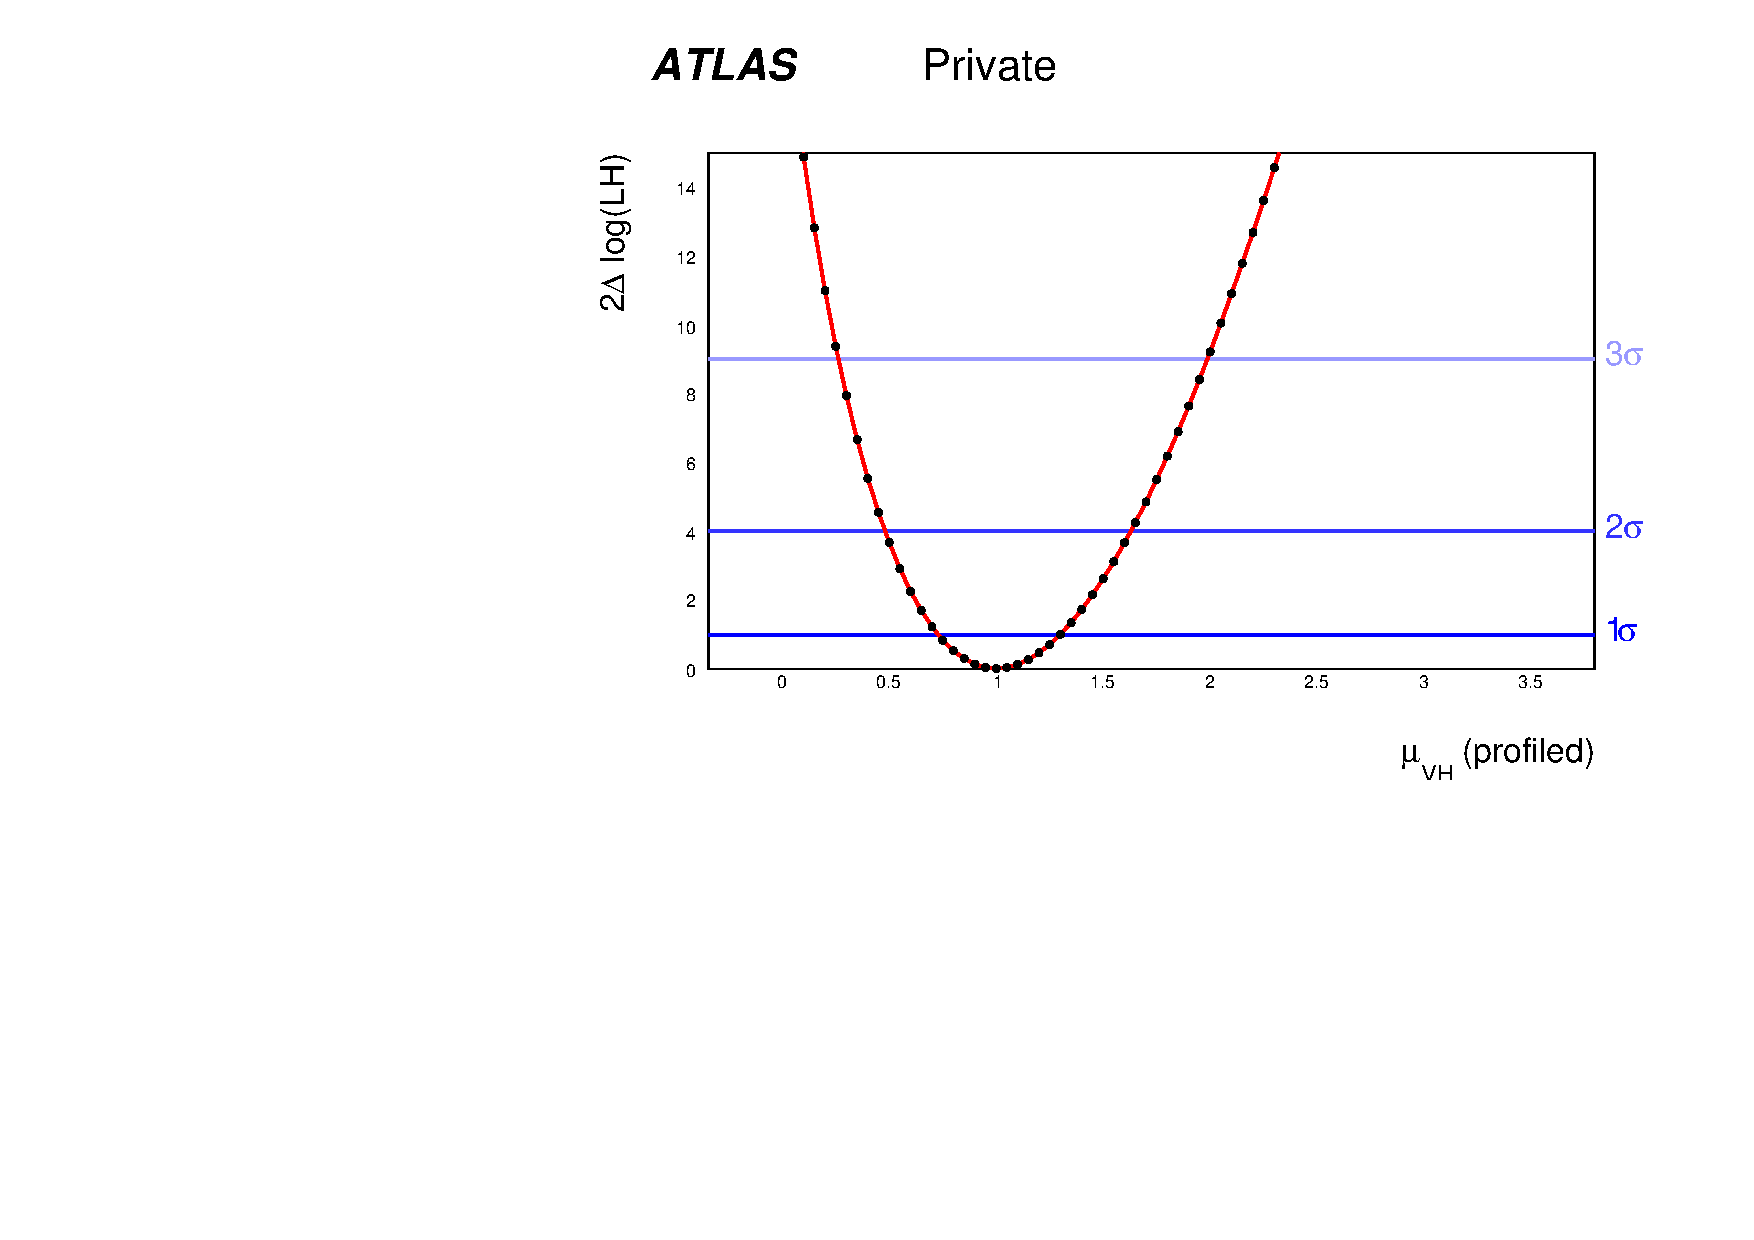
\includegraphics[width=0.6\linewidth]{figures/statistical/nll_plots_vh_expected.pdf}
  }
  \caption{Expected likelihood scans for the \vh{} results.}\label{fig:vh_likelihood_scan}
\end{figure}

The impact of statistical and systematic uncertainties of the \vh{} measurement is assessed through the pulls and nuisance parameter ranking as seen in Appendix~\ref{app:vh_pull_plots}, and the correlations between uncertainties as shown in Appendix~\ref{app:vh_correlation_plots}.

All results from the \vh{} channel are summarized in Table~\ref{tab:vh_inclusive_results_summary}. As expected, the measurement is dominated by statistical uncertainties.

\begin{table}[htp]
  \centering
  % Top row: two tables side by side
  \begin{minipage}{0.48\textwidth}
    \centering
    \begin{tabular}{l|c}
      \hline
      \multicolumn{2}{c}{\textbf{Results Summary}} \\
      \hline
      $\mu_{VH}$ (Expected) & $1.00^{+0.29}_{-0.29}$ \\
      \hline
      Significance (Expected) & $4.45\sigma$ \\
      \hline
    \end{tabular}
  \end{minipage}
  \hfill
  \caption{Summary of the expected and observed signal strengths and significances for the \vh{} inclusive fit}\label{tab:vh_inclusive_results_summary}
\end{table}